\hypertarget{mrshellprim_8c}{
\section{mrshellprim.c File Reference}
\label{mrshellprim_8c}\index{mrshellprim.c@{mrshellprim.c}}
}
{\tt \#include $<$stdio.h$>$}\par
{\tt \#include $<$string.h$>$}\par
{\tt \#include $<$errno.h$>$}\par
{\tt \#include \char`\"{}mrshellprim.h\char`\"{}}\par


Include dependency graph for mrshellprim.c:\begin{figure}[H]
\begin{center}
\leavevmode
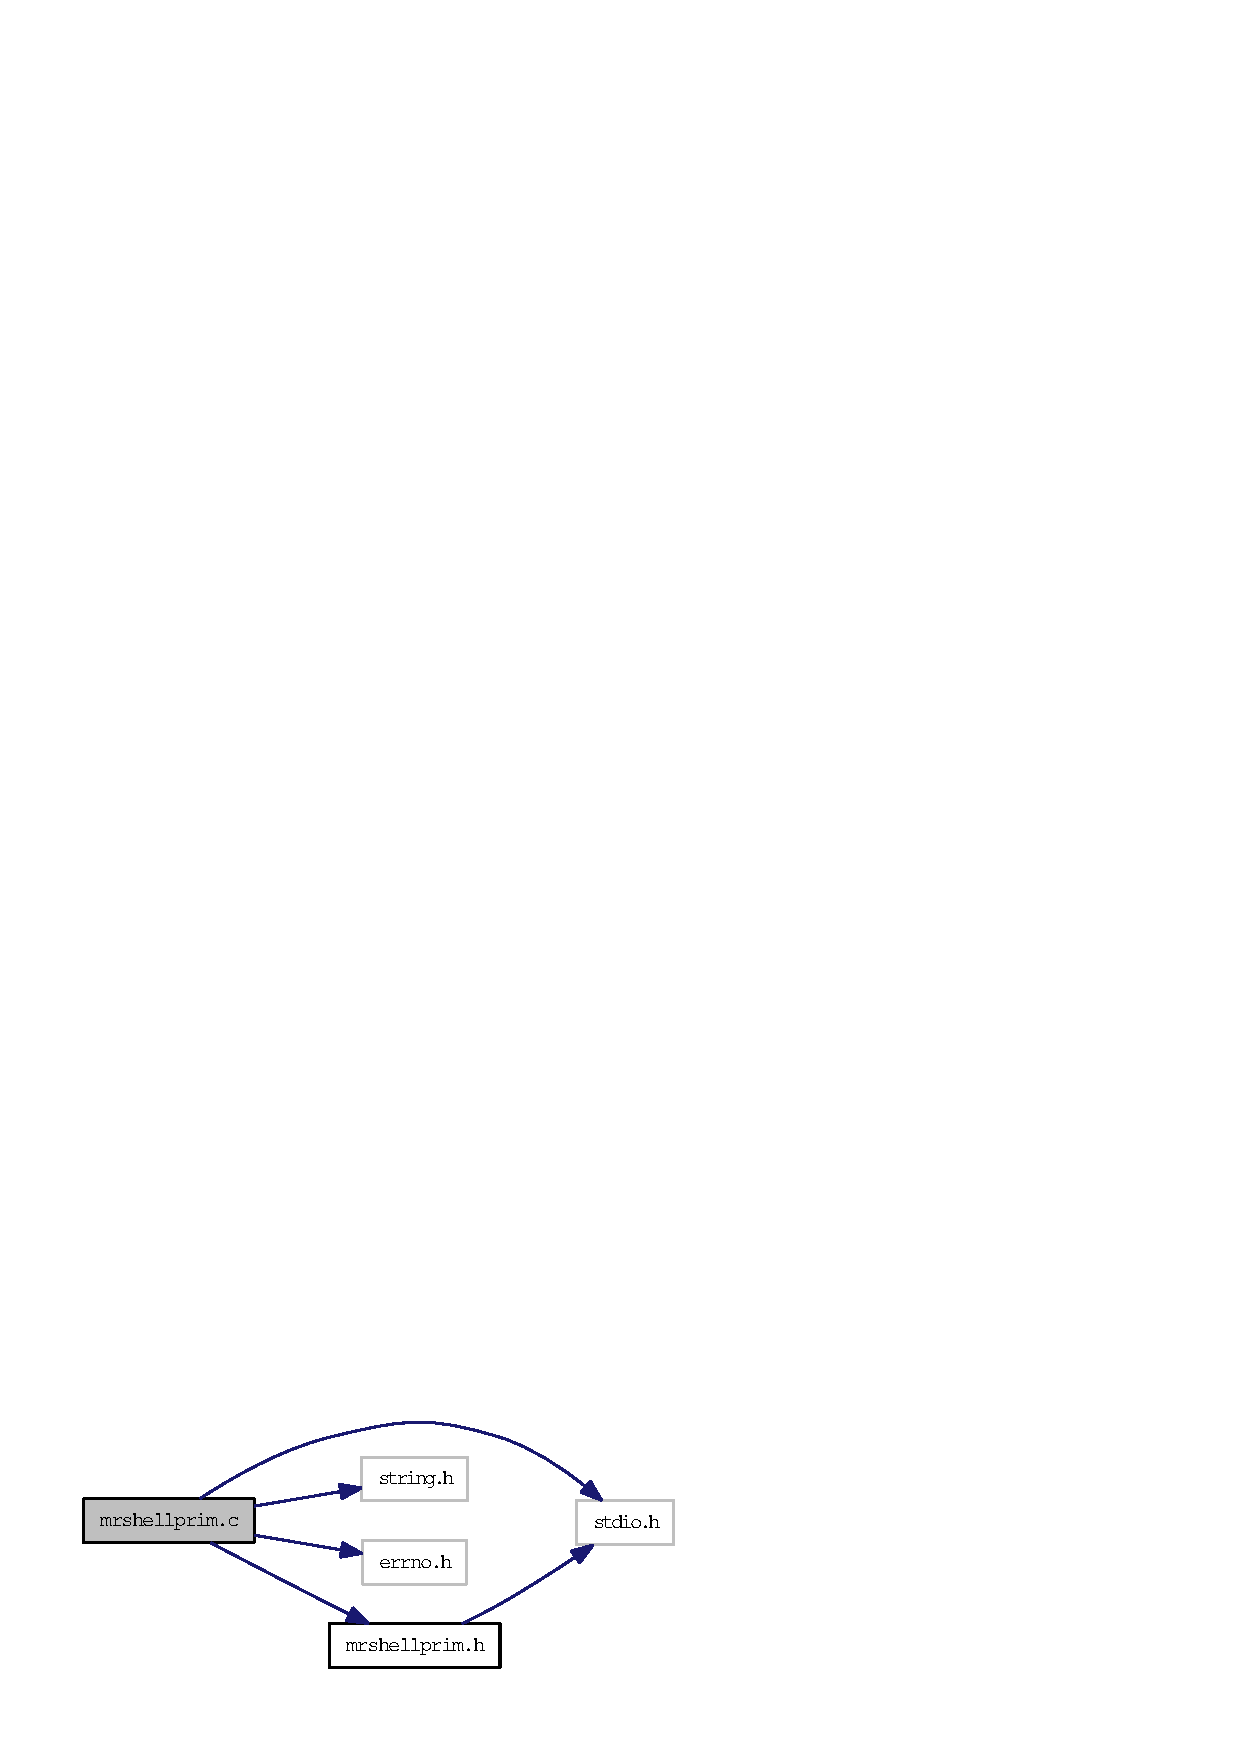
\includegraphics[width=164pt]{mrshellprim_8c__incl}
\end{center}
\end{figure}
\subsection*{Defines}
\begin{CompactItemize}
\item 
\#define \hyperlink{mrshellprim_8c_db27d0beb974602604e269d3efcdb71d}{ARGPROC\_\-FOUND}~0x1000
\begin{CompactList}\small\item\em the argument was found \item\end{CompactList}\item 
\#define \hyperlink{mrshellprim_8c_ca324a1333271c0a90fd93f2233f6de4}{ARGPROC\_\-FAILED}~0x2000
\begin{CompactList}\small\item\em the argument was found, but additional argument scan failed \item\end{CompactList}\end{CompactItemize}
\subsection*{Functions}
\begin{CompactItemize}
\item 
char $\ast$ \hyperlink{mrshellprim_8c_e8ed3396fcb78ea4adce3d902b77541a}{remove\-Prec\-And\-Trailing\-Spec\-Chars} (char $\ast$p\-Cmd)
\begin{CompactList}\small\item\em Remove preceeding and trailing special characters and blanks. \item\end{CompactList}\item 
int \hyperlink{mrshellprim_8c_0244dae55f177bb00bfae3a0a39f6f5a}{get\-Hex\-Number\-From\-Arg} (const char $\ast$arg, unsigned int $\ast$p\-Number, int b\-Warning)
\begin{CompactList}\small\item\em Scan a string for a hex number. \item\end{CompactList}\item 
int \hyperlink{mrshellprim_8c_fe29afcd7e0ed24611394b379523e597}{get\-Dec\-Number\-From\-Arg} (const char $\ast$arg, int $\ast$p\-Number, int b\-Warning)
\begin{CompactList}\small\item\em Scan a string for a decimal number. \item\end{CompactList}\item 
int \hyperlink{mrshellprim_8c_bd0f88fefc2b7fb8ffa459b09018c921}{get\-Float\-Number\-From\-Arg} (const char $\ast$arg, float $\ast$p\-Number, int b\-Warning)
\begin{CompactList}\small\item\em Scan a string for a float number. \item\end{CompactList}\item 
int \hyperlink{mrshellprim_8c_cce515828d3fce502c94ea42d622bff4}{build\-Arguments\-From\-Command\-Line} (char $\ast$p\-Cmd\-Line, char $\ast$$\ast$p\-Target\-Array, int i\-Array\-Size, int b\-Separate, int i\-Debug\-Flag)
\begin{CompactList}\small\item\em Scan a buffer of characters, separate commands and extract pointers to single command parameters. \item\end{CompactList}\item 
int \hyperlink{mrshellprim_8c_a6f9bd761fef55fb0f9b33282fe34f1c}{Is\-Separator} (char c, const char $\ast$p\-Delimiters)
\item 
int \hyperlink{mrshellprim_8c_2d0938d152be65a53ca257fe6fa69dc5}{Read\-Argument} (const char $\ast$$\ast$array\-Arg, int i\-Nof\-Args, int i\-First\-Arg\-Start, \hyperlink{structArgDef__t}{TArg\-Def} $\ast$p\-Def, unsigned int flags)
\item 
int \hyperlink{mrshellprim_8c_18f04bffa1754658c42d2aca468f9b2c}{call\-Command\-Handler} (const char $\ast$$\ast$array\-Arg, int i\-Nof\-Args, int i\-First\-Arg\-Start, \hyperlink{structArgDef__t}{TArg\-Def} $\ast$p\-Def, unsigned int flags)
\item 
int \hyperlink{mrshellprim_8c_165feb129efb27e98051dd34ac03f6a4}{Search\-Def} (const char $\ast$p\-Arg, \hyperlink{structArgDef__t}{TArg\-Def} $\ast$array\-Def, \hyperlink{structFctMode__t}{TFct\-Mode} $\ast$p\-Mode)
\item 
int \hyperlink{mrshellprim_8c_d50cc0ad50efa63a876cee5ef7caed9f}{Print\-Argument\-Definition} (\hyperlink{structArgDef__t}{TArg\-Def} $\ast$array\-Def, int b\-All)
\begin{CompactList}\small\item\em Print a summury on the argument definition structure. \item\end{CompactList}\item 
int \hyperlink{mrshellprim_8c_adf119666e05c73934d586afdb6b2462}{Get\-Nof\-Required\-Args} (\hyperlink{structArgDef__t}{TArg\-Def} $\ast$p\-Def)
\item 
int \hyperlink{mrshellprim_8c_e2735ecedc52b1199ecf8a208339c072}{Scan\-Arguments} (const char $\ast$$\ast$array\-Arg, int i\-Nof\-Args, int i\-First\-Arg\-Start, \hyperlink{structArgDef__t}{TArg\-Def} $\ast$array\-Def, \hyperlink{structFctMode__t}{TFct\-Mode} $\ast$p\-Mode)
\begin{CompactList}\small\item\em Scan a list or single string of arguments. \item\end{CompactList}\item 
unsigned int \hyperlink{mrshellprim_8c_84fd8dd7e4af266b7b6a400c0cacaea4}{mr\-Shell\-Prim\-Set\-Debug\-Flag} (unsigned int flag)
\begin{CompactList}\small\item\em Set a debug flag for the parser. \item\end{CompactList}\item 
unsigned int \hyperlink{mrshellprim_8c_1d4f9511ebb635164beca6c9a4a52756}{mr\-Shell\-Prim\-Clear\-Debug\-Flag} (unsigned int flag)
\begin{CompactList}\small\item\em Clear a debug flag for the parser. \item\end{CompactList}\item 
int \hyperlink{mrshellprim_8c_20b23f294fae687b7b0ad7c6483ec564}{mr\-Shell\-Prim\-Print\-Dbg\-Flags} ()
\begin{CompactList}\small\item\em Print help information on the parser debug flags. \item\end{CompactList}\item 
int \hyperlink{mrshellprim_8c_24d874900c59cf760f128ae366f7a72e}{mr\-Shell\-Prim\-Get\-Index} (\hyperlink{structArgDef__t}{TArg\-Def} $\ast$array\-Def, const char $\ast$p\-Cmd, int i\-Type)
\begin{CompactList}\small\item\em Search the argument definition for a command. \item\end{CompactList}\item 
int \hyperlink{mrshellprim_8c_9f0fe9837b7198fea2f3c32bcf203ed9}{mr\-Shell\-Prim\-Set\-Data} (\hyperlink{structArgDef__t}{TArg\-Def} $\ast$array\-Def, const char $\ast$p\-Cmd, void $\ast$p\-Data, int i\-Type)
\begin{CompactList}\small\item\em Set data pointer for an argument definition element. \item\end{CompactList}\item 
int \hyperlink{mrshellprim_8c_aa038cf5a29f51145c876af7fb5271d3}{mr\-Shell\-Prim\-Get\-Data} (\hyperlink{structArgDef__t}{TArg\-Def} $\ast$array\-Def, const char $\ast$p\-Cmd, void $\ast$$\ast$pp\-Data, int i\-Type)
\begin{CompactList}\small\item\em Get data pointer for an argument definition element. \item\end{CompactList}\item 
int \hyperlink{mrshellprim_8c_1e963c0f8d38ab1305d075b016de0a65}{mr\-Shell\-Prim\-Get\-Float} (\hyperlink{structArgDef__t}{TArg\-Def} $\ast$array\-Def, const char $\ast$p\-Cmd, float $\ast$p\-Float)
\begin{CompactList}\small\item\em Get float value for an argument definition element. \item\end{CompactList}\item 
int \hyperlink{mrshellprim_8c_8f73442602070f02c40b4b3e32ab61a3}{mr\-Shell\-Prim\-Get\-Int} (\hyperlink{structArgDef__t}{TArg\-Def} $\ast$array\-Def, const char $\ast$p\-Cmd, int $\ast$p\-Int)
\begin{CompactList}\small\item\em Get integer value for an argument definition element. \item\end{CompactList}\item 
int \hyperlink{mrshellprim_8c_c08c7b1e961204b98f9b29120f043c6c}{mr\-Shell\-Prim\-Get\-Hex} (\hyperlink{structArgDef__t}{TArg\-Def} $\ast$array\-Def, const char $\ast$p\-Cmd, unsigned int $\ast$p\-Hex)
\begin{CompactList}\small\item\em Get hexadecimal value for an argument definition element. \item\end{CompactList}\item 
\hyperlink{structArgDef__t}{TArg\-Def} $\ast$ \hyperlink{mrshellprim_8c_60d2a9ecd4a849eaf72375ffeb666769}{mr\-Shell\-Prim\-Clone\-Def} (\hyperlink{structArgDef__t}{TArg\-Def} $\ast$array\-Def)
\begin{CompactList}\small\item\em Clone an argument definition. \item\end{CompactList}\item 
int \hyperlink{mrshellprim_8c_e24662763dc15a9b4719cc0f3d98f8fc}{mr\-Shell\-Prim\-Reset\-Volatile\-Flags} (\hyperlink{structArgDef__t}{TArg\-Def} $\ast$array\-Def)
\begin{CompactList}\small\item\em Reset volatile processing flags of the definition array. \item\end{CompactList}\end{CompactItemize}
\subsection*{Variables}
\begin{CompactItemize}
\item 
unsigned int \hyperlink{mrshellprim_8c_34fcfc606a53070425a87fce190ee38d}{g\_\-mr\-Shell\-Prim\-Dbg} = 0x0
\end{CompactItemize}


\subsection{Define Documentation}
\hypertarget{mrshellprim_8c_ca324a1333271c0a90fd93f2233f6de4}{
\index{mrshellprim.c@{mrshellprim.c}!ARGPROC_FAILED@{ARGPROC\_\-FAILED}}
\index{ARGPROC_FAILED@{ARGPROC\_\-FAILED}!mrshellprim.c@{mrshellprim.c}}
\subsubsection[ARGPROC\_\-FAILED]{\setlength{\rightskip}{0pt plus 5cm}\#define ARGPROC\_\-FAILED~0x2000}}
\label{mrshellprim_8c_ca324a1333271c0a90fd93f2233f6de4}


the argument was found, but additional argument scan failed 



Definition at line 42 of file mrshellprim.c.

Referenced by mr\-Shell\-Prim\-Reset\-Volatile\-Flags(), Scan\-Arguments(), and Search\-Def().\hypertarget{mrshellprim_8c_db27d0beb974602604e269d3efcdb71d}{
\index{mrshellprim.c@{mrshellprim.c}!ARGPROC_FOUND@{ARGPROC\_\-FOUND}}
\index{ARGPROC_FOUND@{ARGPROC\_\-FOUND}!mrshellprim.c@{mrshellprim.c}}
\subsubsection[ARGPROC\_\-FOUND]{\setlength{\rightskip}{0pt plus 5cm}\#define ARGPROC\_\-FOUND~0x1000}}
\label{mrshellprim_8c_db27d0beb974602604e269d3efcdb71d}


the argument was found 



Definition at line 40 of file mrshellprim.c.

Referenced by mr\-Shell\-Prim\-Get\-Data(), mr\-Shell\-Prim\-Get\-Float(), mr\-Shell\-Prim\-Get\-Hex(), mr\-Shell\-Prim\-Get\-Int(), mr\-Shell\-Prim\-Reset\-Volatile\-Flags(), Print\-Argument\-Definition(), Scan\-Arguments(), and Search\-Def().

\subsection{Function Documentation}
\hypertarget{mrshellprim_8c_cce515828d3fce502c94ea42d622bff4}{
\index{mrshellprim.c@{mrshellprim.c}!buildArgumentsFromCommandLine@{buildArgumentsFromCommandLine}}
\index{buildArgumentsFromCommandLine@{buildArgumentsFromCommandLine}!mrshellprim.c@{mrshellprim.c}}
\subsubsection[buildArgumentsFromCommandLine]{\setlength{\rightskip}{0pt plus 5cm}int build\-Arguments\-From\-Command\-Line (char $\ast$ {\em p\-Cmd\-Line}, char $\ast$$\ast$ {\em p\-Target\-Array}, int {\em i\-Array\-Size}, int {\em b\-Separate}, int {\em i\-Debug\-Flag})}}
\label{mrshellprim_8c_cce515828d3fce502c94ea42d622bff4}


Scan a buffer of characters, separate commands and extract pointers to single command parameters. 

\begin{Desc}
\item[Parameters:]
\begin{description}
\item[{\em p\-Cmd\-Line}]pointer to zero terminated input char buffer, the content is changed if b\-Separate==1!!! \item[{\em p\-Target\-Array}]array to receive pointers to separated strings \item[{\em i\-Array\-Size}]size of the target array \item[{\em b\-Separate}]blanks and special characters set to zero to separate two command parameters \end{description}
\end{Desc}
\begin{Desc}
\item[Returns:]number of parameters if succeeded, pointers to separated strings in taget array\par
 neg. error code if failed \end{Desc}


Definition at line 128 of file mrshellprim.c.

References DBG\_\-ARGUMENT\_\-CONVERT.

Referenced by execute\-Command\-Line().\hypertarget{mrshellprim_8c_18f04bffa1754658c42d2aca468f9b2c}{
\index{mrshellprim.c@{mrshellprim.c}!callCommandHandler@{callCommandHandler}}
\index{callCommandHandler@{callCommandHandler}!mrshellprim.c@{mrshellprim.c}}
\subsubsection[callCommandHandler]{\setlength{\rightskip}{0pt plus 5cm}int call\-Command\-Handler (const char $\ast$$\ast$ {\em array\-Arg}, int {\em i\-Nof\-Args}, int {\em i\-First\-Arg\-Start}, \hyperlink{structArgDef__t}{TArg\-Def} $\ast$ {\em p\-Def}, unsigned int {\em flags})}}
\label{mrshellprim_8c_18f04bffa1754658c42d2aca468f9b2c}




Definition at line 357 of file mrshellprim.c.

References Arg\-Def\_\-t::data, DBG\_\-SCAN\_\-ARG\_\-DEF, e\-Bool, e\-Char\-Array, e\-Composite, e\-Const\-String, e\-Fct\-Arg\-Def, e\-Fct\-Composite\-Args, e\-Fct\-Float\-Args, e\-Fct\-Hex\-Args, e\-Fct\-Inclusive, e\-Fct\-Index, e\-Fct\-Integer\-Args, e\-Fct\-No\-Arg, e\-Fct\-Remaining, e\-Fct\-User\-Scan, e\-Flag, e\-Float, e\-Float\-Array, e\-Hex, e\-Hex\-Array, e\-Integer, e\-Integer\-Array, g\_\-mr\-Shell\-Prim\-Dbg, Tagged\-Data\_\-t::Int, Arg\-Def\_\-t::l, Fct\-Arg\_\-t::p\-Def, Arg\-Def\_\-t::p\-Fct\-Arg, Tagged\-Data\_\-t::p\-Fct\-Arg\-Def, Tagged\-Data\_\-t::p\-Fct\-Index, Arg\-Def\_\-t::p\-Fct\-Mode, Tagged\-Data\_\-t::p\-Fct\-No\-Arg, Tagged\-Data\_\-t::p\-Fct\-User, Tagged\-Data\_\-t::p\-Int, Fct\-Arg\_\-t::p\-Mode, Tagged\-Data\_\-t::p\-Sub\-Arg\-Def, Fct\-Arg\_\-t::p\-User, Arg\-Def\_\-t::p\-User, Arg\-Def\_\-t::s, Scan\-Arguments(), Arg\-Def\_\-t::set\-Flag\-Pattern, Arg\-Def\_\-t::size, and Tagged\-Data\_\-t::type.

Referenced by Scan\-Arguments().

Here is the call graph for this function:\begin{figure}[H]
\begin{center}
\leavevmode
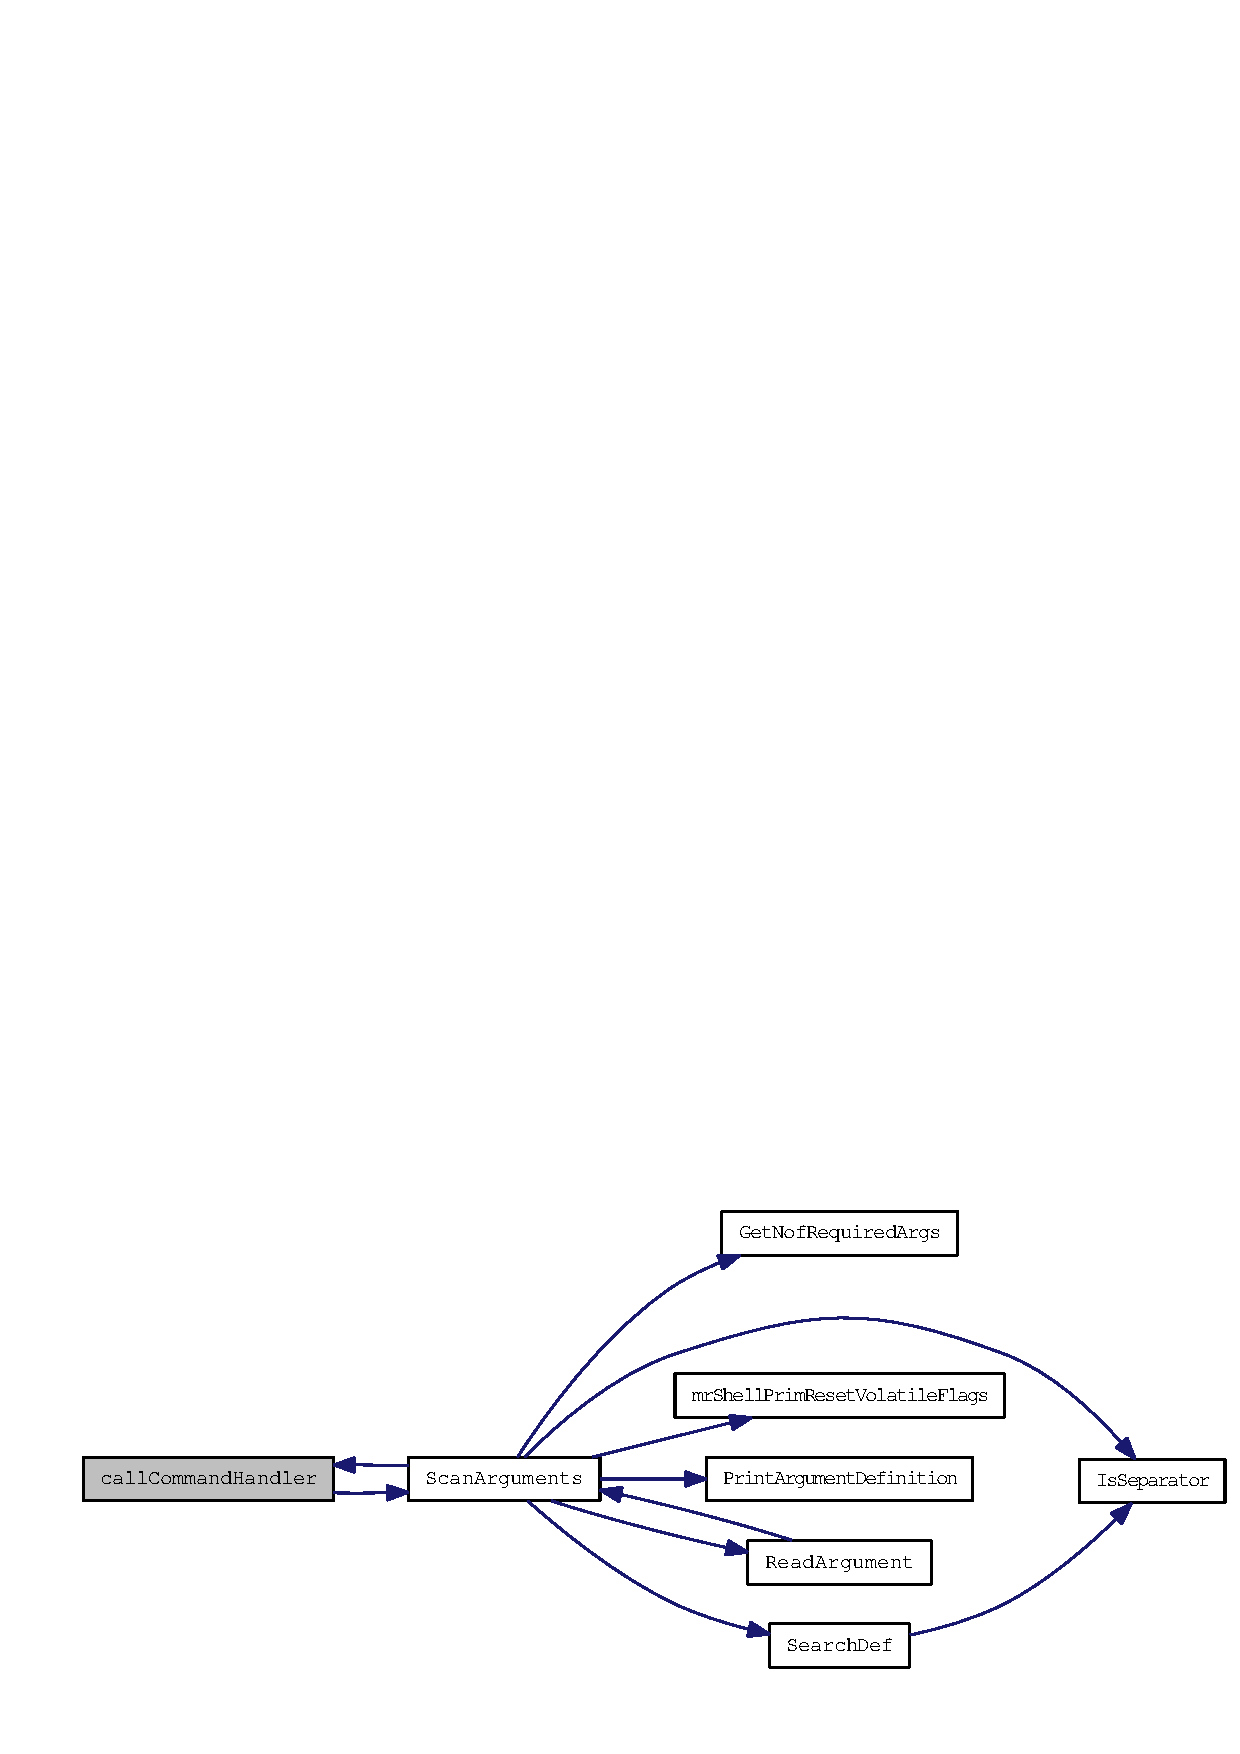
\includegraphics[width=296pt]{mrshellprim_8c_18f04bffa1754658c42d2aca468f9b2c_cgraph}
\end{center}
\end{figure}
\hypertarget{mrshellprim_8c_fe29afcd7e0ed24611394b379523e597}{
\index{mrshellprim.c@{mrshellprim.c}!getDecNumberFromArg@{getDecNumberFromArg}}
\index{getDecNumberFromArg@{getDecNumberFromArg}!mrshellprim.c@{mrshellprim.c}}
\subsubsection[getDecNumberFromArg]{\setlength{\rightskip}{0pt plus 5cm}int get\-Dec\-Number\-From\-Arg (const char $\ast$ {\em arg}, int $\ast$ {\em p\-Number}, int {\em b\-Warning})}}
\label{mrshellprim_8c_fe29afcd7e0ed24611394b379523e597}


Scan a string for a decimal number. 

\begin{Desc}
\item[Parameters:]
\begin{description}
\item[{\em arg}]the string \item[{\em p\-Number}]target to receive the decimal number \item[{\em b\-Warning}]display a warning if argument could not be converted \end{description}
\end{Desc}
\begin{Desc}
\item[Returns:]$>$=0 if succeeded, neg. error code if failed \end{Desc}


Definition at line 84 of file mrshellprim.c.

Referenced by build\-Data\-Buffer\-From\-File(), exec\-Batch(), exec\-Read\-Cmd(), exec\-Reg\-Read\-Cmd(), exec\-Reg\-Write\-Cmd(), execute\-Main\-Commands(), and exec\-Write\-Cmd().\hypertarget{mrshellprim_8c_bd0f88fefc2b7fb8ffa459b09018c921}{
\index{mrshellprim.c@{mrshellprim.c}!getFloatNumberFromArg@{getFloatNumberFromArg}}
\index{getFloatNumberFromArg@{getFloatNumberFromArg}!mrshellprim.c@{mrshellprim.c}}
\subsubsection[getFloatNumberFromArg]{\setlength{\rightskip}{0pt plus 5cm}int get\-Float\-Number\-From\-Arg (const char $\ast$ {\em arg}, float $\ast$ {\em p\-Number}, int {\em b\-Warning})}}
\label{mrshellprim_8c_bd0f88fefc2b7fb8ffa459b09018c921}


Scan a string for a float number. 

\begin{Desc}
\item[Parameters:]
\begin{description}
\item[{\em arg}]the string \item[{\em p\-Number}]target to receive the float number \item[{\em b\-Warning}]display a warning if argument could not be converted \end{description}
\end{Desc}
\begin{Desc}
\item[Returns:]$>$=0 if succeeded, neg. error code if failed \end{Desc}


Definition at line 101 of file mrshellprim.c.

Referenced by Scan\-Coefficients().\hypertarget{mrshellprim_8c_0244dae55f177bb00bfae3a0a39f6f5a}{
\index{mrshellprim.c@{mrshellprim.c}!getHexNumberFromArg@{getHexNumberFromArg}}
\index{getHexNumberFromArg@{getHexNumberFromArg}!mrshellprim.c@{mrshellprim.c}}
\subsubsection[getHexNumberFromArg]{\setlength{\rightskip}{0pt plus 5cm}int get\-Hex\-Number\-From\-Arg (const char $\ast$ {\em arg}, unsigned int $\ast$ {\em p\-Number}, int {\em b\-Warning})}}
\label{mrshellprim_8c_0244dae55f177bb00bfae3a0a39f6f5a}


Scan a string for a hex number. 

\begin{Desc}
\item[Parameters:]
\begin{description}
\item[{\em arg}]the string \item[{\em p\-Number}]target to receive the hex number \item[{\em b\-Warning}]display a warning if argument could not be converted \end{description}
\end{Desc}
\begin{Desc}
\item[Returns:]$>$=0 if succeeded, neg. error code if failed \end{Desc}


Definition at line 67 of file mrshellprim.c.

Referenced by exec\-Read\-Cmd(), exec\-Reg\-Write\-Cmd(), execute\-Main\-Commands(), exec\-Write\-Cmd(), Scan\-Coefficients(), and wait\-Condition().\hypertarget{mrshellprim_8c_adf119666e05c73934d586afdb6b2462}{
\index{mrshellprim.c@{mrshellprim.c}!GetNofRequiredArgs@{GetNofRequiredArgs}}
\index{GetNofRequiredArgs@{GetNofRequiredArgs}!mrshellprim.c@{mrshellprim.c}}
\subsubsection[GetNofRequiredArgs]{\setlength{\rightskip}{0pt plus 5cm}int Get\-Nof\-Required\-Args (\hyperlink{structArgDef__t}{TArg\-Def} $\ast$ {\em p\-Def})}}
\label{mrshellprim_8c_adf119666e05c73934d586afdb6b2462}




Definition at line 653 of file mrshellprim.c.

References Arg\-Def\_\-t::array\-Composite, Arg\-Def\_\-t::data, DBG\_\-SCAN\_\-ARG\_\-DEF\_\-DETAIL, e\-Char\-Array, e\-Const\-String, e\-Fct\-Arg\-Def, e\-Fct\-Composite\-Args, e\-Fct\-Float\-Args, e\-Fct\-Hex\-Args, e\-Fct\-Integer\-Args, e\-Float, e\-Float\-Array, e\-Hex, e\-Hex\-Array, e\-Integer, e\-Integer\-Array, e\-Unknown\-Type, g\_\-mr\-Shell\-Prim\-Dbg, Arg\-Def\_\-t::size, and Tagged\-Data\_\-t::type.

Referenced by Scan\-Arguments().\hypertarget{mrshellprim_8c_a6f9bd761fef55fb0f9b33282fe34f1c}{
\index{mrshellprim.c@{mrshellprim.c}!IsSeparator@{IsSeparator}}
\index{IsSeparator@{IsSeparator}!mrshellprim.c@{mrshellprim.c}}
\subsubsection[IsSeparator]{\setlength{\rightskip}{0pt plus 5cm}int Is\-Separator (char {\em c}, const char $\ast$ {\em p\-Delimiters})}}
\label{mrshellprim_8c_a6f9bd761fef55fb0f9b33282fe34f1c}




Definition at line 207 of file mrshellprim.c.

References DBG\_\-SCAN\_\-ARG\_\-DEF\_\-DETAIL, and g\_\-mr\-Shell\-Prim\-Dbg.

Referenced by Scan\-Arguments(), and Search\-Def().\hypertarget{mrshellprim_8c_1d4f9511ebb635164beca6c9a4a52756}{
\index{mrshellprim.c@{mrshellprim.c}!mrShellPrimClearDebugFlag@{mrShellPrimClearDebugFlag}}
\index{mrShellPrimClearDebugFlag@{mrShellPrimClearDebugFlag}!mrshellprim.c@{mrshellprim.c}}
\subsubsection[mrShellPrimClearDebugFlag]{\setlength{\rightskip}{0pt plus 5cm}unsigned int mr\-Shell\-Prim\-Clear\-Debug\-Flag (unsigned int {\em flag})}}
\label{mrshellprim_8c_1d4f9511ebb635164beca6c9a4a52756}


Clear a debug flag for the parser. 

\begin{Desc}
\item[Parameters:]
\begin{description}
\item[{\em flag}]the flag set set \end{description}
\end{Desc}
\begin{Desc}
\item[Returns:]the current value of the flags \end{Desc}


Definition at line 960 of file mrshellprim.c.

References g\_\-mr\-Shell\-Prim\-Dbg.\hypertarget{mrshellprim_8c_60d2a9ecd4a849eaf72375ffeb666769}{
\index{mrshellprim.c@{mrshellprim.c}!mrShellPrimCloneDef@{mrShellPrimCloneDef}}
\index{mrShellPrimCloneDef@{mrShellPrimCloneDef}!mrshellprim.c@{mrshellprim.c}}
\subsubsection[mrShellPrimCloneDef]{\setlength{\rightskip}{0pt plus 5cm}\hyperlink{structArgDef__t}{TArg\-Def}$\ast$ mr\-Shell\-Prim\-Clone\-Def (\hyperlink{structArgDef__t}{TArg\-Def} $\ast$ {\em array\-Def})}}
\label{mrshellprim_8c_60d2a9ecd4a849eaf72375ffeb666769}


Clone an argument definition. 

\begin{Desc}
\item[Parameters:]
\begin{description}
\item[{\em array\-Def}]pointer to definition array, terminated by \hyperlink{mrshellprim_8h_76a810650461f2062938ee9b82666b36a94b1781ada88507c56c4475f25fa92f}{e\-Unknown\-Type} element \end{description}
\end{Desc}
\begin{Desc}
\item[Returns:]pointer to new definition array\par
 The allocated memory has to be released by the caller \end{Desc}


Definition at line 1082 of file mrshellprim.c.

References Arg\-Def\_\-t::data, e\-Unknown\-Type, and Tagged\-Data\_\-t::type.

Referenced by execute\-Command\-Args().\hypertarget{mrshellprim_8c_aa038cf5a29f51145c876af7fb5271d3}{
\index{mrshellprim.c@{mrshellprim.c}!mrShellPrimGetData@{mrShellPrimGetData}}
\index{mrShellPrimGetData@{mrShellPrimGetData}!mrshellprim.c@{mrshellprim.c}}
\subsubsection[mrShellPrimGetData]{\setlength{\rightskip}{0pt plus 5cm}int mr\-Shell\-Prim\-Get\-Data (\hyperlink{structArgDef__t}{TArg\-Def} $\ast$ {\em array\-Def}, const char $\ast$ {\em p\-Cmd}, void $\ast$$\ast$ {\em pp\-Data}, int {\em i\-Type})}}
\label{mrshellprim_8c_aa038cf5a29f51145c876af7fb5271d3}


Get data pointer for an argument definition element. 

The function is only available for other arguments than of type \hyperlink{mrshellprim_8h_76a810650461f2062938ee9b82666b36dd647739976fe8f17c25e3fe04d30eeb}{e\-Integer}, e\-Bool, i\-Float and i\-Hex. \begin{Desc}
\item[Parameters:]
\begin{description}
\item[{\em array\-Def}]argument definition array, terminated by an element of type \hyperlink{mrshellprim_8h_76a810650461f2062938ee9b82666b36a94b1781ada88507c56c4475f25fa92f}{e\-Unknown\-Type} \item[{\em p\-Cmd}]command string, both the short and the long definition are compared \item[{\em p\-Float}]data target \item[{\em pp\-Data}]pointer to void pointer to receive data pointer \item[{\em i\-Type}]if not equal to e\-Unknown\-Type a type check is done \end{description}
\end{Desc}
\begin{Desc}
\item[Returns:]$>$=0 success, index of the element in lower 16bit; bit 16 set if this argument was found.\par
 the ARGPROC\_\-INDEX and ARGPROC\_\-EXISTS macros can be used to extract to parts\par
 neg. error code if failed\par
 -ENOENT entry not found\par
 -EBADF entry found, but of wrong type\par
 -EINVAL invalid argument\par
 -ENOSYS function not available for this type\par
 \end{Desc}


Definition at line 1019 of file mrshellprim.c.

References ARGPROC\_\-EXISTS\_\-BITSHIFT, ARGPROC\_\-FOUND, Arg\-Def\_\-t::data, e\-Bool, e\-Float, e\-Hex, e\-Integer, mr\-Shell\-Prim\-Get\-Index(), Tagged\-Data\_\-t::p\-Void, and Tagged\-Data\_\-t::type.

Referenced by main().

Here is the call graph for this function:\begin{figure}[H]
\begin{center}
\leavevmode
\includegraphics[width=154pt]{mrshellprim_8c_aa038cf5a29f51145c876af7fb5271d3_cgraph}
\end{center}
\end{figure}
\hypertarget{mrshellprim_8c_1e963c0f8d38ab1305d075b016de0a65}{
\index{mrshellprim.c@{mrshellprim.c}!mrShellPrimGetFloat@{mrShellPrimGetFloat}}
\index{mrShellPrimGetFloat@{mrShellPrimGetFloat}!mrshellprim.c@{mrshellprim.c}}
\subsubsection[mrShellPrimGetFloat]{\setlength{\rightskip}{0pt plus 5cm}int mr\-Shell\-Prim\-Get\-Float (\hyperlink{structArgDef__t}{TArg\-Def} $\ast$ {\em array\-Def}, const char $\ast$ {\em p\-Cmd}, float $\ast$ {\em p\-Float})}}
\label{mrshellprim_8c_1e963c0f8d38ab1305d075b016de0a65}


Get float value for an argument definition element. 

The function is only available arguments of type i\-Float. \begin{Desc}
\item[Parameters:]
\begin{description}
\item[{\em array\-Def}]argument definition array, terminated by an element of type \hyperlink{mrshellprim_8h_76a810650461f2062938ee9b82666b36a94b1781ada88507c56c4475f25fa92f}{e\-Unknown\-Type} \item[{\em p\-Cmd}]command string, both the short and the long definition are compared \item[{\em p\-Float}]data target \end{description}
\end{Desc}
\begin{Desc}
\item[Returns:]$>$=0 success, index of the element in lower 16bit; bit 16 set if this argument was found.\par
 the ARGPROC\_\-INDEX and ARGPROC\_\-EXISTS macros can be used to extract to parts\par
 neg. error code if failed\par
 -ENOENT entry not found\par
 -EBADF entry found, but of wrong type\par
 -EINVAL invalid argument\par
 -ENOSYS function not available for this type\par
 \end{Desc}


Definition at line 1040 of file mrshellprim.c.

References ARGPROC\_\-EXISTS\_\-BITSHIFT, ARGPROC\_\-FOUND, Arg\-Def\_\-t::data, e\-Float, Tagged\-Data\_\-t::Float, and mr\-Shell\-Prim\-Get\-Index().

Here is the call graph for this function:\begin{figure}[H]
\begin{center}
\leavevmode
\includegraphics[width=154pt]{mrshellprim_8c_1e963c0f8d38ab1305d075b016de0a65_cgraph}
\end{center}
\end{figure}
\hypertarget{mrshellprim_8c_c08c7b1e961204b98f9b29120f043c6c}{
\index{mrshellprim.c@{mrshellprim.c}!mrShellPrimGetHex@{mrShellPrimGetHex}}
\index{mrShellPrimGetHex@{mrShellPrimGetHex}!mrshellprim.c@{mrshellprim.c}}
\subsubsection[mrShellPrimGetHex]{\setlength{\rightskip}{0pt plus 5cm}int mr\-Shell\-Prim\-Get\-Hex (\hyperlink{structArgDef__t}{TArg\-Def} $\ast$ {\em array\-Def}, const char $\ast$ {\em p\-Cmd}, unsigned int $\ast$ {\em p\-Hex})}}
\label{mrshellprim_8c_c08c7b1e961204b98f9b29120f043c6c}


Get hexadecimal value for an argument definition element. 

The function is only available for arguments of type i\-Hex \begin{Desc}
\item[Parameters:]
\begin{description}
\item[{\em array\-Def}]argument definition array, terminated by an element of type \hyperlink{mrshellprim_8h_76a810650461f2062938ee9b82666b36a94b1781ada88507c56c4475f25fa92f}{e\-Unknown\-Type} \item[{\em p\-Cmd}]command string, both the short and the long definition are compared \item[{\em p\-Hex}]data target \end{description}
\end{Desc}
\begin{Desc}
\item[Returns:]$>$=0 success, index of the element in lower 16bit; bit 16 set if this argument was found.\par
 the ARGPROC\_\-INDEX and ARGPROC\_\-EXISTS macros can be used to extract to parts\par
 neg. error code if failed\par
 -ENOENT entry not found\par
 -EBADF entry found, but of wrong type\par
 -EINVAL invalid argument\par
 -ENOSYS function not available for this type\par
 \end{Desc}


Definition at line 1070 of file mrshellprim.c.

References ARGPROC\_\-EXISTS\_\-BITSHIFT, ARGPROC\_\-FOUND, Arg\-Def\_\-t::data, e\-Hex, Tagged\-Data\_\-t::Hex, and mr\-Shell\-Prim\-Get\-Index().

Referenced by driver\-Ctrl\-Cmds(), exec\-Flash\-Erase(), and main().

Here is the call graph for this function:\begin{figure}[H]
\begin{center}
\leavevmode
\includegraphics[width=152pt]{mrshellprim_8c_c08c7b1e961204b98f9b29120f043c6c_cgraph}
\end{center}
\end{figure}
\hypertarget{mrshellprim_8c_24d874900c59cf760f128ae366f7a72e}{
\index{mrshellprim.c@{mrshellprim.c}!mrShellPrimGetIndex@{mrShellPrimGetIndex}}
\index{mrShellPrimGetIndex@{mrShellPrimGetIndex}!mrshellprim.c@{mrshellprim.c}}
\subsubsection[mrShellPrimGetIndex]{\setlength{\rightskip}{0pt plus 5cm}int mr\-Shell\-Prim\-Get\-Index (\hyperlink{structArgDef__t}{TArg\-Def} $\ast$ {\em array\-Def}, const char $\ast$ {\em p\-Cmd}, int {\em i\-Type})}}
\label{mrshellprim_8c_24d874900c59cf760f128ae366f7a72e}


Search the argument definition for a command. 

\begin{Desc}
\item[Parameters:]
\begin{description}
\item[{\em array\-Def}]argument definition array, terminated by an element of type \hyperlink{mrshellprim_8h_76a810650461f2062938ee9b82666b36a94b1781ada88507c56c4475f25fa92f}{e\-Unknown\-Type} \item[{\em p\-Cmd}]command string, both the short and the long definition are compared \item[{\em i\-Type}]if not equal to e\-Unknown\-Type a type check is done \end{description}
\end{Desc}
\begin{Desc}
\item[Returns:]$>$=0 success, index of the element neg. error code if failed\par
 -ENOENT entry not found\par
 -EBADF entry found, but of wrong type\par
 -EINVAL invalid argument\par
 \end{Desc}


Definition at line 979 of file mrshellprim.c.

References Arg\-Def\_\-t::data, e\-Unknown\-Type, and Tagged\-Data\_\-t::type.

Referenced by mr\-Shell\-Prim\-Get\-Data(), mr\-Shell\-Prim\-Get\-Float(), mr\-Shell\-Prim\-Get\-Hex(), mr\-Shell\-Prim\-Get\-Int(), and mr\-Shell\-Prim\-Set\-Data().\hypertarget{mrshellprim_8c_8f73442602070f02c40b4b3e32ab61a3}{
\index{mrshellprim.c@{mrshellprim.c}!mrShellPrimGetInt@{mrShellPrimGetInt}}
\index{mrShellPrimGetInt@{mrShellPrimGetInt}!mrshellprim.c@{mrshellprim.c}}
\subsubsection[mrShellPrimGetInt]{\setlength{\rightskip}{0pt plus 5cm}int mr\-Shell\-Prim\-Get\-Int (\hyperlink{structArgDef__t}{TArg\-Def} $\ast$ {\em array\-Def}, const char $\ast$ {\em p\-Cmd}, int $\ast$ {\em p\-Int})}}
\label{mrshellprim_8c_8f73442602070f02c40b4b3e32ab61a3}


Get integer value for an argument definition element. 

The function is only available arguments of type i\-Integer and e\-Bool. \begin{Desc}
\item[Parameters:]
\begin{description}
\item[{\em array\-Def}]argument definition array, terminated by an element of type \hyperlink{mrshellprim_8h_76a810650461f2062938ee9b82666b36a94b1781ada88507c56c4475f25fa92f}{e\-Unknown\-Type} \item[{\em p\-Cmd}]command string, both the short and the long definition are compared \item[{\em p\-Int}]data target \end{description}
\end{Desc}
\begin{Desc}
\item[Returns:]$>$=0 success, index of the element in lower 16bit; bit 16 set if this argument was found.\par
 the ARGPROC\_\-INDEX and ARGPROC\_\-EXISTS macros can be used to extract to parts\par
 neg. error code if failed\par
 -ENOENT entry not found\par
 -EBADF entry found, but of wrong type\par
 -EINVAL invalid argument\par
 -ENOSYS function not available for this type\par
 \end{Desc}


Definition at line 1052 of file mrshellprim.c.

References ARGPROC\_\-EXISTS\_\-BITSHIFT, ARGPROC\_\-FOUND, Arg\-Def\_\-t::data, e\-Bool, e\-Integer, e\-Unknown\-Type, Tagged\-Data\_\-t::Int, mr\-Shell\-Prim\-Get\-Index(), and Tagged\-Data\_\-t::type.

Referenced by exec\-Flash\-Erase(), and main().

Here is the call graph for this function:\begin{figure}[H]
\begin{center}
\leavevmode
\includegraphics[width=149pt]{mrshellprim_8c_8f73442602070f02c40b4b3e32ab61a3_cgraph}
\end{center}
\end{figure}
\hypertarget{mrshellprim_8c_20b23f294fae687b7b0ad7c6483ec564}{
\index{mrshellprim.c@{mrshellprim.c}!mrShellPrimPrintDbgFlags@{mrShellPrimPrintDbgFlags}}
\index{mrShellPrimPrintDbgFlags@{mrShellPrimPrintDbgFlags}!mrshellprim.c@{mrshellprim.c}}
\subsubsection[mrShellPrimPrintDbgFlags]{\setlength{\rightskip}{0pt plus 5cm}int mr\-Shell\-Prim\-Print\-Dbg\-Flags ()}}
\label{mrshellprim_8c_20b23f294fae687b7b0ad7c6483ec564}


Print help information on the parser debug flags. 



Definition at line 966 of file mrshellprim.c.

References DBG\_\-ARGUMENT\_\-CONVERT, DBG\_\-ARGUMENT\_\-READ, DBG\_\-SCAN\_\-ARG\_\-DEF, DBG\_\-SCAN\_\-ARG\_\-DEF\_\-DETAIL, DBG\_\-SEARCH\_\-ARG\_\-DEF, and DBG\_\-SEARCH\_\-ARG\_\-DEF\_\-DETAIL.\hypertarget{mrshellprim_8c_e24662763dc15a9b4719cc0f3d98f8fc}{
\index{mrshellprim.c@{mrshellprim.c}!mrShellPrimResetVolatileFlags@{mrShellPrimResetVolatileFlags}}
\index{mrShellPrimResetVolatileFlags@{mrShellPrimResetVolatileFlags}!mrshellprim.c@{mrshellprim.c}}
\subsubsection[mrShellPrimResetVolatileFlags]{\setlength{\rightskip}{0pt plus 5cm}int mr\-Shell\-Prim\-Reset\-Volatile\-Flags (\hyperlink{structArgDef__t}{TArg\-Def} $\ast$ {\em array\-Def})}}
\label{mrshellprim_8c_e24662763dc15a9b4719cc0f3d98f8fc}


Reset volatile processing flags of the definition array. 

Reseted flags: \hyperlink{mrshellprim_8c_db27d0beb974602604e269d3efcdb71d}{ARGPROC\_\-FOUND} \begin{Desc}
\item[Parameters:]
\begin{description}
\item[{\em array\-Def}]pointer to definition array, terminated by \hyperlink{mrshellprim_8h_76a810650461f2062938ee9b82666b36a94b1781ada88507c56c4475f25fa92f}{e\-Unknown\-Type} element \end{description}
\end{Desc}
\begin{Desc}
\item[Returns:]$>$=0 success, neg. error code if failed \end{Desc}


Definition at line 1098 of file mrshellprim.c.

References ARGPROC\_\-FAILED, ARGPROC\_\-FOUND, Arg\-Def\_\-t::data, e\-Unknown\-Type, and Tagged\-Data\_\-t::type.

Referenced by Scan\-Arguments().\hypertarget{mrshellprim_8c_9f0fe9837b7198fea2f3c32bcf203ed9}{
\index{mrshellprim.c@{mrshellprim.c}!mrShellPrimSetData@{mrShellPrimSetData}}
\index{mrShellPrimSetData@{mrShellPrimSetData}!mrshellprim.c@{mrshellprim.c}}
\subsubsection[mrShellPrimSetData]{\setlength{\rightskip}{0pt plus 5cm}int mr\-Shell\-Prim\-Set\-Data (\hyperlink{structArgDef__t}{TArg\-Def} $\ast$ {\em array\-Def}, const char $\ast$ {\em p\-Cmd}, void $\ast$ {\em p\-Data}, int {\em i\-Type})}}
\label{mrshellprim_8c_9f0fe9837b7198fea2f3c32bcf203ed9}


Set data pointer for an argument definition element. 

The function is only available for other arguments than of type \hyperlink{mrshellprim_8h_76a810650461f2062938ee9b82666b36dd647739976fe8f17c25e3fe04d30eeb}{e\-Integer}, e\-Bool, i\-Float and i\-Hex. \begin{Desc}
\item[Parameters:]
\begin{description}
\item[{\em array\-Def}]argument definition array, terminated by an element of type \hyperlink{mrshellprim_8h_76a810650461f2062938ee9b82666b36a94b1781ada88507c56c4475f25fa92f}{e\-Unknown\-Type} \item[{\em p\-Cmd}]command string, both the short and the long definition are compared \item[{\em p\-Data}]void pointer to data \item[{\em i\-Type}]if not equal to e\-Unknown\-Type a type check is done \end{description}
\end{Desc}
\begin{Desc}
\item[Returns:]$>$=0 success, index of the element in lower 16bit neg. error code if failed\par
 -ENOENT entry not found\par
 -EBADF entry found, but of wrong type\par
 -EINVAL invalid argument\par
 -ENOSYS function not available for this type\par
 \end{Desc}


Definition at line 1005 of file mrshellprim.c.

References Arg\-Def\_\-t::data, e\-Bool, e\-Float, e\-Hex, e\-Integer, mr\-Shell\-Prim\-Get\-Index(), Tagged\-Data\_\-t::p\-Void, and Tagged\-Data\_\-t::type.

Here is the call graph for this function:\begin{figure}[H]
\begin{center}
\leavevmode
\includegraphics[width=153pt]{mrshellprim_8c_9f0fe9837b7198fea2f3c32bcf203ed9_cgraph}
\end{center}
\end{figure}
\hypertarget{mrshellprim_8c_84fd8dd7e4af266b7b6a400c0cacaea4}{
\index{mrshellprim.c@{mrshellprim.c}!mrShellPrimSetDebugFlag@{mrShellPrimSetDebugFlag}}
\index{mrShellPrimSetDebugFlag@{mrShellPrimSetDebugFlag}!mrshellprim.c@{mrshellprim.c}}
\subsubsection[mrShellPrimSetDebugFlag]{\setlength{\rightskip}{0pt plus 5cm}unsigned int mr\-Shell\-Prim\-Set\-Debug\-Flag (unsigned int {\em flag})}}
\label{mrshellprim_8c_84fd8dd7e4af266b7b6a400c0cacaea4}


Set a debug flag for the parser. 

\begin{Desc}
\item[Parameters:]
\begin{description}
\item[{\em flag}]the flag set set \end{description}
\end{Desc}
\begin{Desc}
\item[Returns:]the current value of the flags \end{Desc}


Definition at line 954 of file mrshellprim.c.

References g\_\-mr\-Shell\-Prim\-Dbg.\hypertarget{mrshellprim_8c_d50cc0ad50efa63a876cee5ef7caed9f}{
\index{mrshellprim.c@{mrshellprim.c}!PrintArgumentDefinition@{PrintArgumentDefinition}}
\index{PrintArgumentDefinition@{PrintArgumentDefinition}!mrshellprim.c@{mrshellprim.c}}
\subsubsection[PrintArgumentDefinition]{\setlength{\rightskip}{0pt plus 5cm}int Print\-Argument\-Definition (\hyperlink{structArgDef__t}{TArg\-Def} $\ast$ {\em array\-Def}, int {\em b\-All})}}
\label{mrshellprim_8c_d50cc0ad50efa63a876cee5ef7caed9f}


Print a summury on the argument definition structure. 

The type and eventually scanned values are printed out together with the flags set for the element. This is a debug feature. \begin{Desc}
\item[Parameters:]
\begin{description}
\item[{\em array\-Def}]argument definition array, terminated by an element of type \hyperlink{mrshellprim_8h_76a810650461f2062938ee9b82666b36a94b1781ada88507c56c4475f25fa92f}{e\-Unknown\-Type} \item[{\em b\-All}]\end{description}
\end{Desc}
\begin{Desc}
\item[Returns:]$>$=0 success, neg. error code if failed \end{Desc}


Definition at line 565 of file mrshellprim.c.

References ARGPROC\_\-FOUND, Arg\-Def\_\-t::data, e\-Bool, e\-Char\-Array, e\-Composite, e\-Const\-String, e\-Fct\-Arg\-Def, e\-Fct\-Composite\-Args, e\-Fct\-Float\-Args, e\-Fct\-Hex\-Args, e\-Fct\-Inclusive, e\-Fct\-Index, e\-Fct\-Integer\-Args, e\-Fct\-No\-Arg, e\-Fct\-Remaining, e\-Fct\-User\-Scan, e\-Flag, e\-Float, e\-Float\-Array, e\-Hex, e\-Hex\-Array, e\-Integer, e\-Integer\-Array, e\-Unknown\-Type, Tagged\-Data\_\-t::p\-String, and Tagged\-Data\_\-t::type.

Referenced by Scan\-Arguments().\hypertarget{mrshellprim_8c_2d0938d152be65a53ca257fe6fa69dc5}{
\index{mrshellprim.c@{mrshellprim.c}!ReadArgument@{ReadArgument}}
\index{ReadArgument@{ReadArgument}!mrshellprim.c@{mrshellprim.c}}
\subsubsection[ReadArgument]{\setlength{\rightskip}{0pt plus 5cm}int Read\-Argument (const char $\ast$$\ast$ {\em array\-Arg}, int {\em i\-Nof\-Args}, int {\em i\-First\-Arg\-Start}, \hyperlink{structArgDef__t}{TArg\-Def} $\ast$ {\em p\-Def}, unsigned int {\em flags})}}
\label{mrshellprim_8c_2d0938d152be65a53ca257fe6fa69dc5}




Definition at line 230 of file mrshellprim.c.

References Arg\-Def\_\-t::data, DBG\_\-ARGUMENT\_\-READ, DBG\_\-SCAN\_\-ARG\_\-DEF, e\-Bool, e\-Char\-Array, e\-Composite, e\-Const\-String, e\-Fct\-Arg\-Def, e\-Fct\-Composite\-Args, e\-Fct\-Float\-Args, e\-Fct\-Hex\-Args, e\-Fct\-Inclusive, e\-Fct\-Index, e\-Fct\-Integer\-Args, e\-Fct\-No\-Arg, e\-Fct\-Remaining, e\-Fct\-User\-Scan, e\-Flag, e\-Float, e\-Float\-Array, e\-Hex, e\-Hex\-Array, e\-Integer, e\-Integer\-Array, Tagged\-Data\_\-t::Float, g\_\-mr\-Shell\-Prim\-Dbg, Tagged\-Data\_\-t::Hex, Tagged\-Data\_\-t::Int, Fct\-Arg\_\-t::p\-Def, Arg\-Def\_\-t::p\-Fct\-Arg, Tagged\-Data\_\-t::p\-Hex, Fct\-Arg\_\-t::p\-Mode, Tagged\-Data\_\-t::p\-String, Scan\-Arguments(), SCANMODE\_\-SILENT, SCANRET\_\-BITSHIFT\_\-OFFSET\_\-LAST\_\-ARG, and Tagged\-Data\_\-t::type.

Referenced by Scan\-Arguments().

Here is the call graph for this function:\begin{figure}[H]
\begin{center}
\leavevmode
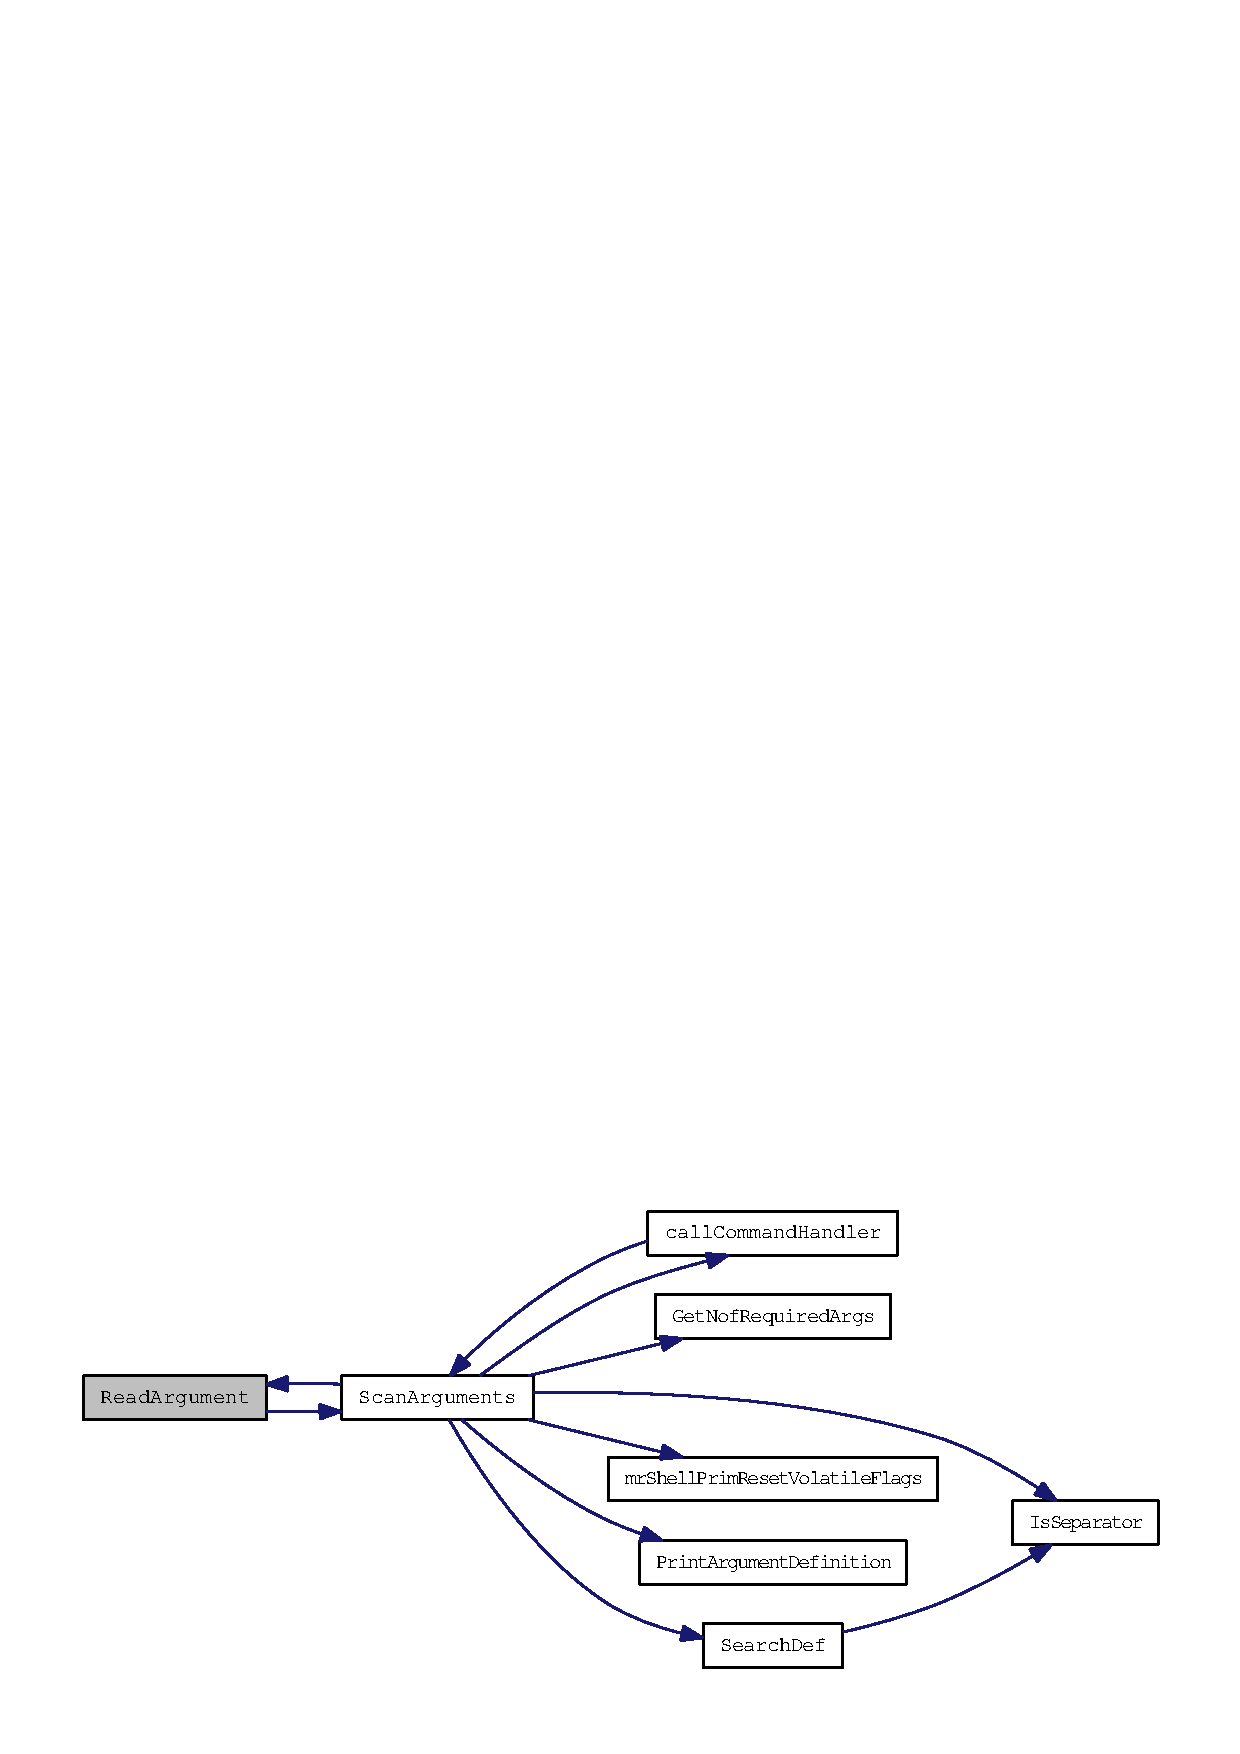
\includegraphics[width=280pt]{mrshellprim_8c_2d0938d152be65a53ca257fe6fa69dc5_cgraph}
\end{center}
\end{figure}
\hypertarget{mrshellprim_8c_e8ed3396fcb78ea4adce3d902b77541a}{
\index{mrshellprim.c@{mrshellprim.c}!removePrecAndTrailingSpecChars@{removePrecAndTrailingSpecChars}}
\index{removePrecAndTrailingSpecChars@{removePrecAndTrailingSpecChars}!mrshellprim.c@{mrshellprim.c}}
\subsubsection[removePrecAndTrailingSpecChars]{\setlength{\rightskip}{0pt plus 5cm}char$\ast$ remove\-Prec\-And\-Trailing\-Spec\-Chars (char $\ast$ {\em p\-Cmd})}}
\label{mrshellprim_8c_e8ed3396fcb78ea4adce3d902b77541a}


Remove preceeding and trailing special characters and blanks. 

Until now the function removes blanks at the beginning and newlines at the end.\par
 {\bf Note:} The function alters the buffer. \begin{Desc}
\item[Parameters:]
\begin{description}
\item[{\em p\-Cmd}]char buffer holding the command \end{description}
\end{Desc}
\begin{Desc}
\item[Returns:]pointer to the first non-special character of the buffer if succeeded \end{Desc}


Definition at line 44 of file mrshellprim.c.

Referenced by exec\-Batch(), and main().\hypertarget{mrshellprim_8c_e2735ecedc52b1199ecf8a208339c072}{
\index{mrshellprim.c@{mrshellprim.c}!ScanArguments@{ScanArguments}}
\index{ScanArguments@{ScanArguments}!mrshellprim.c@{mrshellprim.c}}
\subsubsection[ScanArguments]{\setlength{\rightskip}{0pt plus 5cm}int Scan\-Arguments (const char $\ast$$\ast$ {\em array\-Arg}, int {\em i\-Nof\-Args}, int {\em i\-First\-Arg\-Start}, \hyperlink{structArgDef__t}{TArg\-Def} $\ast$ {\em array\-Def}, \hyperlink{structFctMode__t}{TFct\-Mode} $\ast$ {\em p\-Mode})}}
\label{mrshellprim_8c_e2735ecedc52b1199ecf8a208339c072}


Scan a list or single string of arguments. 

with respect to the definitions of arguments as entries in the definition array, sub-functions can be called and float, decimal and hexadecimal values can be read \begin{Desc}
\item[Parameters:]
\begin{description}
\item[{\em array\-Arg}]array of argument strings \item[{\em i\-Nof\-Args}]size of the array \item[{\em i\-First\-Arg\-Start}]start of scan within the first element of the array \item[{\em p\-Separator}]a zero terminated string with additional separators, the  value is always treated as separator \item[{\em array\-Def}]an array of TArg\-Def elements, each defining a known argument type \item[{\em flags}]\end{description}
\end{Desc}
\begin{Desc}
\item[Returns:]$>$=0 successfull, offset coded\par
 bit 8-15: number of scanned elements of arg\-Array\par
 bit 0-7: offset in last processed element\par
 -EINTR if an argument with ARGDEF\_\-TERMINATE or ARGDEF\_\-BREAK was found \end{Desc}


Definition at line 692 of file mrshellprim.c.

References ARGDEF\_\-BREAK, ARGDEF\_\-DELAY\_\-EXECUTE, ARGDEF\_\-EXIT, ARGDEF\_\-RESUME, ARGDEF\_\-TERMINATE, ARGPROC\_\-FAILED, ARGPROC\_\-FOUND, call\-Command\-Handler(), DBG\_\-SCAN\_\-ARG\_\-DEF, DBG\_\-SCAN\_\-ARG\_\-DEF\_\-DETAIL, e\-Const\-String, e\-Fct\-Arg\-Def, e\-Fct\-Inclusive, Fct\-Mode\_\-t::flags, Arg\-Def\_\-t::flags, g\_\-mr\-Shell\-Prim\-Dbg, Get\-Nof\-Required\-Args(), Is\-Separator(), Arg\-Def\_\-t::l, mr\-Shell\-Prim\-Reset\-Volatile\-Flags(), Fct\-Mode\_\-t::p\-Delimiters, Print\-Argument\-Definition(), Read\-Argument(), Arg\-Def\_\-t::s, SCANMODE\_\-FORCE\_\-TERMINATION, SCANMODE\_\-PERSISTENT, SCANMODE\_\-PRINT\_\-UKWN\_\-SEQU, SCANMODE\_\-READ\_\-ONE\_\-CMD, SCANMODE\_\-SILENT, SCANMODE\_\-SKIP\_\-UKWN\_\-SEQU, SCANRET\_\-BITSHIFT\_\-INDEX, SCANRET\_\-BITSHIFT\_\-OFFSET\_\-LAST\_\-ARG, SCANRET\_\-BITSHIFT\_\-PROCESSED\_\-ARGS, SCANRET\_\-INVAL\_\-INDEX, SCANRET\_\-MASK\_\-INDEX, SCANRET\_\-MASK\_\-OFFSET\_\-LAST\_\-ARG, SCANRET\_\-MASK\_\-PROCESSED\_\-ARGS, and Search\-Def().

Referenced by call\-Command\-Handler(), execute\-Command\-Args(), main(), and Read\-Argument().

Here is the call graph for this function:\begin{figure}[H]
\begin{center}
\leavevmode
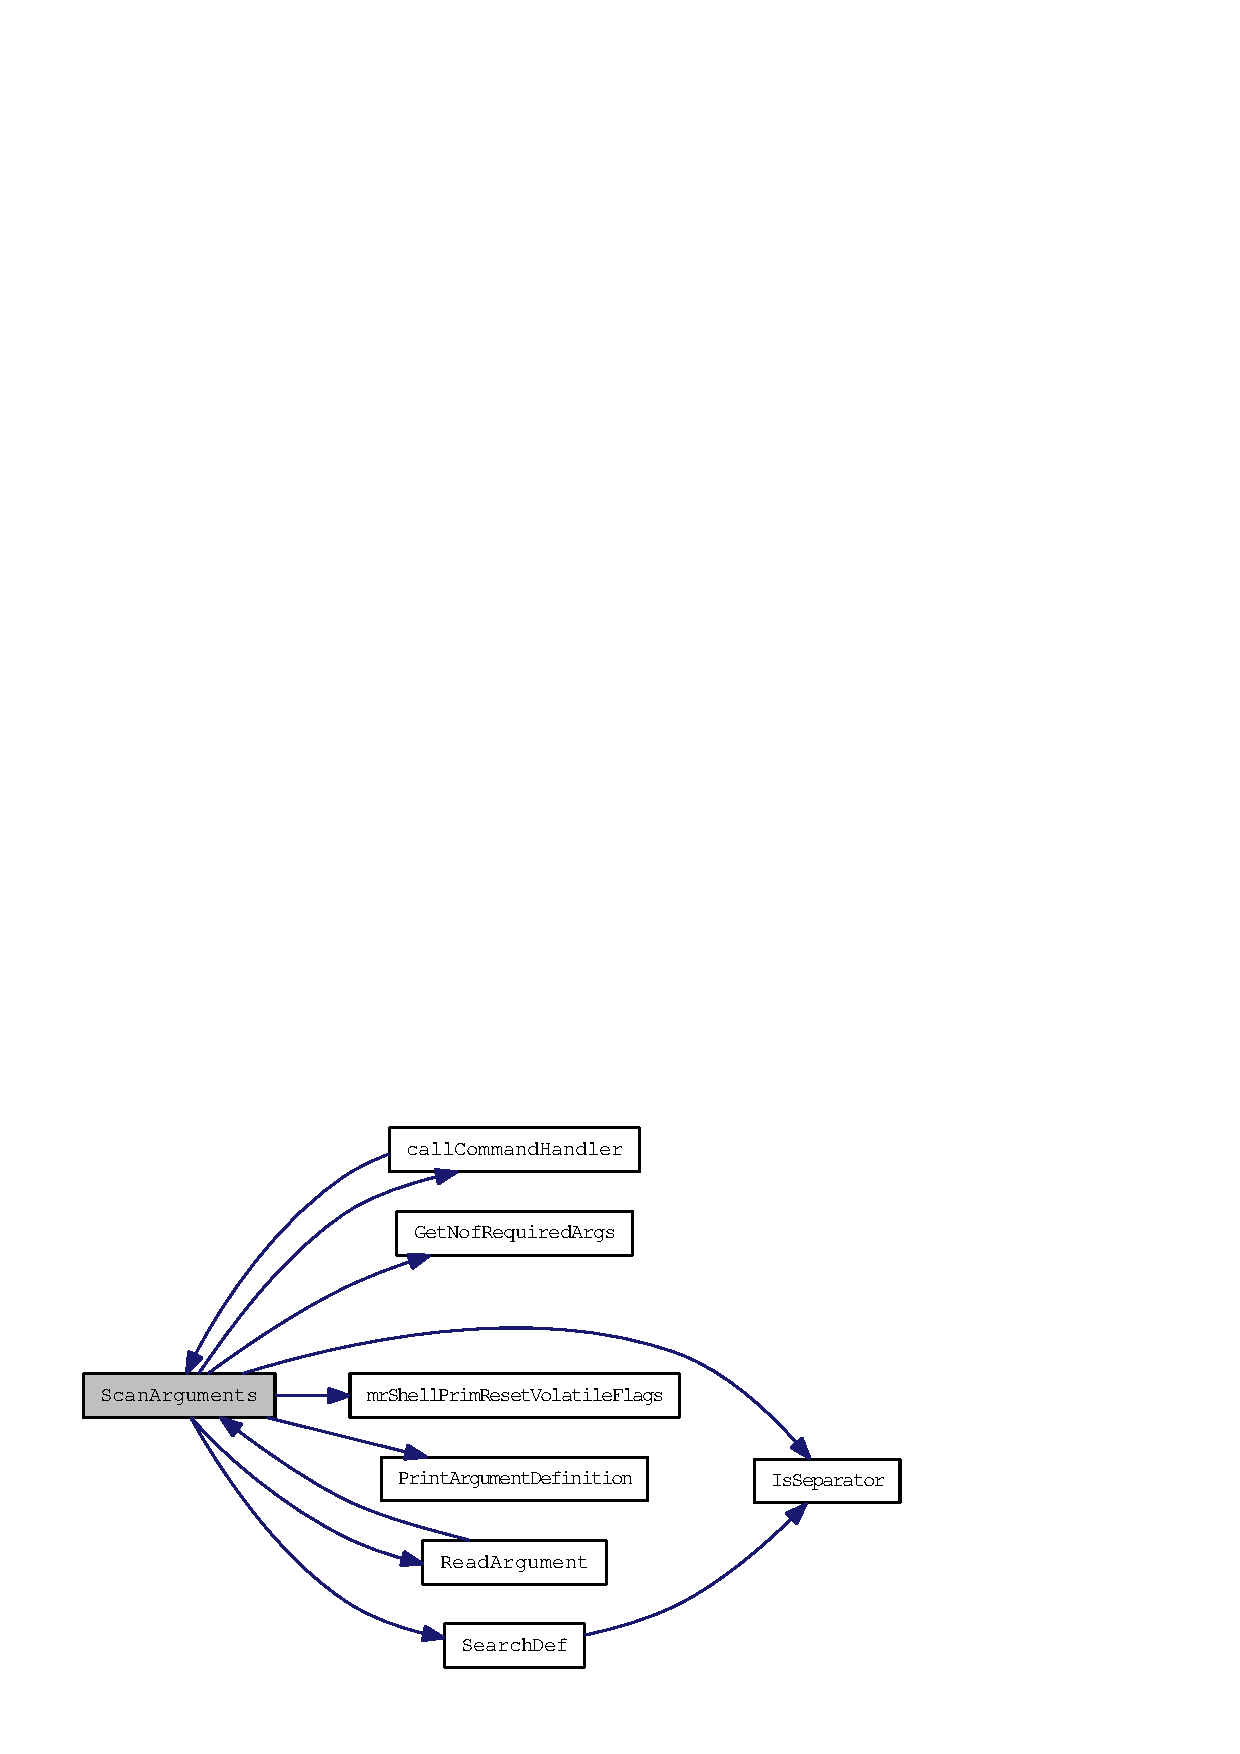
\includegraphics[width=218pt]{mrshellprim_8c_e2735ecedc52b1199ecf8a208339c072_cgraph}
\end{center}
\end{figure}
\hypertarget{mrshellprim_8c_165feb129efb27e98051dd34ac03f6a4}{
\index{mrshellprim.c@{mrshellprim.c}!SearchDef@{SearchDef}}
\index{SearchDef@{SearchDef}!mrshellprim.c@{mrshellprim.c}}
\subsubsection[SearchDef]{\setlength{\rightskip}{0pt plus 5cm}int Search\-Def (const char $\ast$ {\em p\-Arg}, \hyperlink{structArgDef__t}{TArg\-Def} $\ast$ {\em array\-Def}, \hyperlink{structFctMode__t}{TFct\-Mode} $\ast$ {\em p\-Mode})}}
\label{mrshellprim_8c_165feb129efb27e98051dd34ac03f6a4}




Definition at line 448 of file mrshellprim.c.

References ARGDEF\_\-KEYWORDLESS, ARGDEF\_\-ONLY\_\-ONCE, ARGDEF\_\-UNTERM\_\-LONG, ARGDEF\_\-UNTERM\_\-SHORT, ARGPROC\_\-FAILED, ARGPROC\_\-FOUND, Arg\-Def\_\-t::data, DBG\_\-SEARCH\_\-ARG\_\-DEF, DBG\_\-SEARCH\_\-ARG\_\-DEF\_\-DETAIL, e\-Unknown\-Type, Arg\-Def\_\-t::flags, Fct\-Mode\_\-t::flags, g\_\-mr\-Shell\-Prim\-Dbg, Is\-Separator(), Arg\-Def\_\-t::l, Fct\-Mode\_\-t::p\-Delimiters, Arg\-Def\_\-t::s, SCANRET\_\-BITSHIFT\_\-INDEX, SCANRET\_\-BITSHIFT\_\-OFFSET\_\-LAST\_\-ARG, and Tagged\-Data\_\-t::type.

Referenced by Scan\-Arguments().

Here is the call graph for this function:\begin{figure}[H]
\begin{center}
\leavevmode
\includegraphics[width=109pt]{mrshellprim_8c_165feb129efb27e98051dd34ac03f6a4_cgraph}
\end{center}
\end{figure}


\subsection{Variable Documentation}
\hypertarget{mrshellprim_8c_34fcfc606a53070425a87fce190ee38d}{
\index{mrshellprim.c@{mrshellprim.c}!g_mrShellPrimDbg@{g\_\-mrShellPrimDbg}}
\index{g_mrShellPrimDbg@{g\_\-mrShellPrimDbg}!mrshellprim.c@{mrshellprim.c}}
\subsubsection[g\_\-mrShellPrimDbg]{\setlength{\rightskip}{0pt plus 5cm}unsigned int \hyperlink{sendRCUcommand_8c_34fcfc606a53070425a87fce190ee38d}{g\_\-mr\-Shell\-Prim\-Dbg} = 0x0}}
\label{mrshellprim_8c_34fcfc606a53070425a87fce190ee38d}




Definition at line 33 of file mrshellprim.c.

Referenced by call\-Command\-Handler(), Get\-Nof\-Required\-Args(), Is\-Separator(), mr\-Shell\-Prim\-Clear\-Debug\-Flag(), mr\-Shell\-Prim\-Set\-Debug\-Flag(), Read\-Argument(), Scan\-Arguments(), and Search\-Def().